\chapter{Preâmbulo Teórico}

Para que possamos fazer uma análise comparativa entre duas estratégias estatísticas, temos que, antes, entender suas diferenças e similaridades, bem como as características dos dados com os quais estamos lidando.

Assim, este capítulo será dividido em duas grandes seções, uma destinada à apresentação das bases de imagens utilizadas, outra destinada à discussão sobre as qualidades dos dados nessas bases.

\section{As bases de dados}

Para o cumprimento desse trabalho, escolhemos duas bases de imagens diferentes, que chamaremos simplesmente Toyama e LIVE.

A base Toyama é, na verdade, chamada \textbf{IRCCyN/IVC-Toyama database (LCD)} e tem acesso franqueado no site ~\cite{Tourancheau2008} do IRCCyN (\emph{Institut de Recherche en Communications et Cybernétique de Nantes}), da Universidade de Nantes, na França.

A base LIVE é, na verdade, chamada \textbf{LIVE Image Quality Assessment Database} e tem acesso também franqueado no site ~\cite{livedb} do LIVE (\emph{Laboratory for Image \& Video Engineering}).

Ambas as bases possuem imagens originais (não degradadas) e um determinado número de imagens degradadas com diferentes tipos e graus de degradação; nosso trabalho se concentra na degradação do tipo JPEG, em todos os graus de degradação apresentados. A Tabela \ref{tab:bds} apresenta as principais características de ambas as bases.

\begin{table}[htb]
	\footnotesize
	\caption[Características das Imagens das Bases de Dados]{Características das Imagens das Bases de Dados}
	\label{tab:bds}
 	\begin{tabular}{ l | c | c } %\toprule[1.5pt]
% \begin{minipage}{\linewidth}
% \centering
% 	\captionof{table}{Características das Imagens nas Bases de Dados} \label{tab:bds}
% 	\begin{tabular}{ l | c | c } %\toprule[1.5pt]
							&	\textbf{Toyama}			&	\textbf{LIVE} 		\\\hline % \midrule
		Número Total de Imagens	$T_i$		&	$98$				&	$204$	  		\\ % \midrule
		Número de Imagens de Referência $I_r$	& 	$14$				&	$29$		  	\\
		Número de Imagens degradadas $I_d$	&	$84$				&	$175$	  		\\
		Resolução das Imagens na base		& 	$768 \times 512$ pixels 		&	$768 \times 512$ pixels 	\\
		Profundidade de cor			&	$24bits/pixel$			&	$24bits/pixel$ 		\\
		Formato das imagens cedidas		&	BMP				&	BMP		  	\\
		Tipo de degradação			&	JPEG				&	JPEG		  	\\
		Graus de degradação aplicados		& $15$, $20$, $27$, $37$, $55$, $79$ 	& 	não informado 		\\
		Diversidade de graus de degradação	&	$6$ taxas			&  	não informado 		\\
		Faixa de valores de avaliação		& 	$[1, 5]$			& 	$[0, 100]$		\\
		Categorias de Qualidade			&	$5$				& 	$5$			\\
		Sessões de Avaliação distintas		&	$1$				& 	$2$			\\
		
%		\bottomrule[1.25pt]
	\end {tabular}\par
	\legend{Fontes: \cite{livedb,Tourancheau2008}}
\end{table}

As figuras \autoref{fig:liveref} e \autoref{fig:livedist} apresentam exemplos de figuras disponíveis na base LIVE; já as figuras \autoref{fig:toyaref} e \autoref{toyadist} provém da base Toyama. As imagens à esquerda são imagens de referência, não-corrompidas, enquanto as da direita já passaram pela compressão JPEG.

\begin{figure}[htb]
 \label{fig:liveex}
 \centering
  \begin{minipage}{0.45\textwidth}
    \centering
    \caption{Imagem de referência LIVE} \label{fig:liveref}
    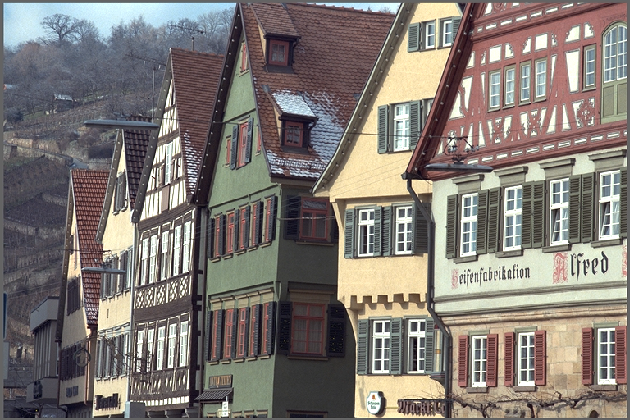
\includegraphics[scale=0.80]{../img/liveref66.pdf}
    \legend{Fonte: \cite{livedb}}
  \end{minipage}
  \hfill
  \begin{minipage}{0.45\textwidth}
    \centering
    \caption{Imagem distorcida LIVE} \label{fig:livedist}
    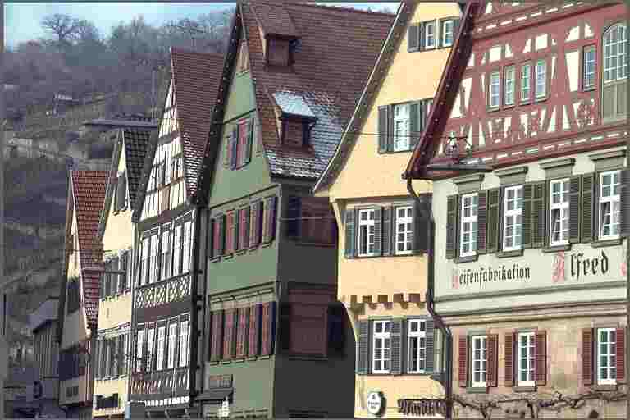
\includegraphics[scale=0.80]{../img/liveref90.pdf}
    \legend{Fonte: \cite{livedb}}
  \end{minipage}
\end{figure}

\begin{figure}[htb]
 \label{fig:toyaex}
 \centering
  \begin{minipage}{0.45\textwidth}
    \centering
    \caption{Imagem de referência Toyama} \label{fig:toyaref}
    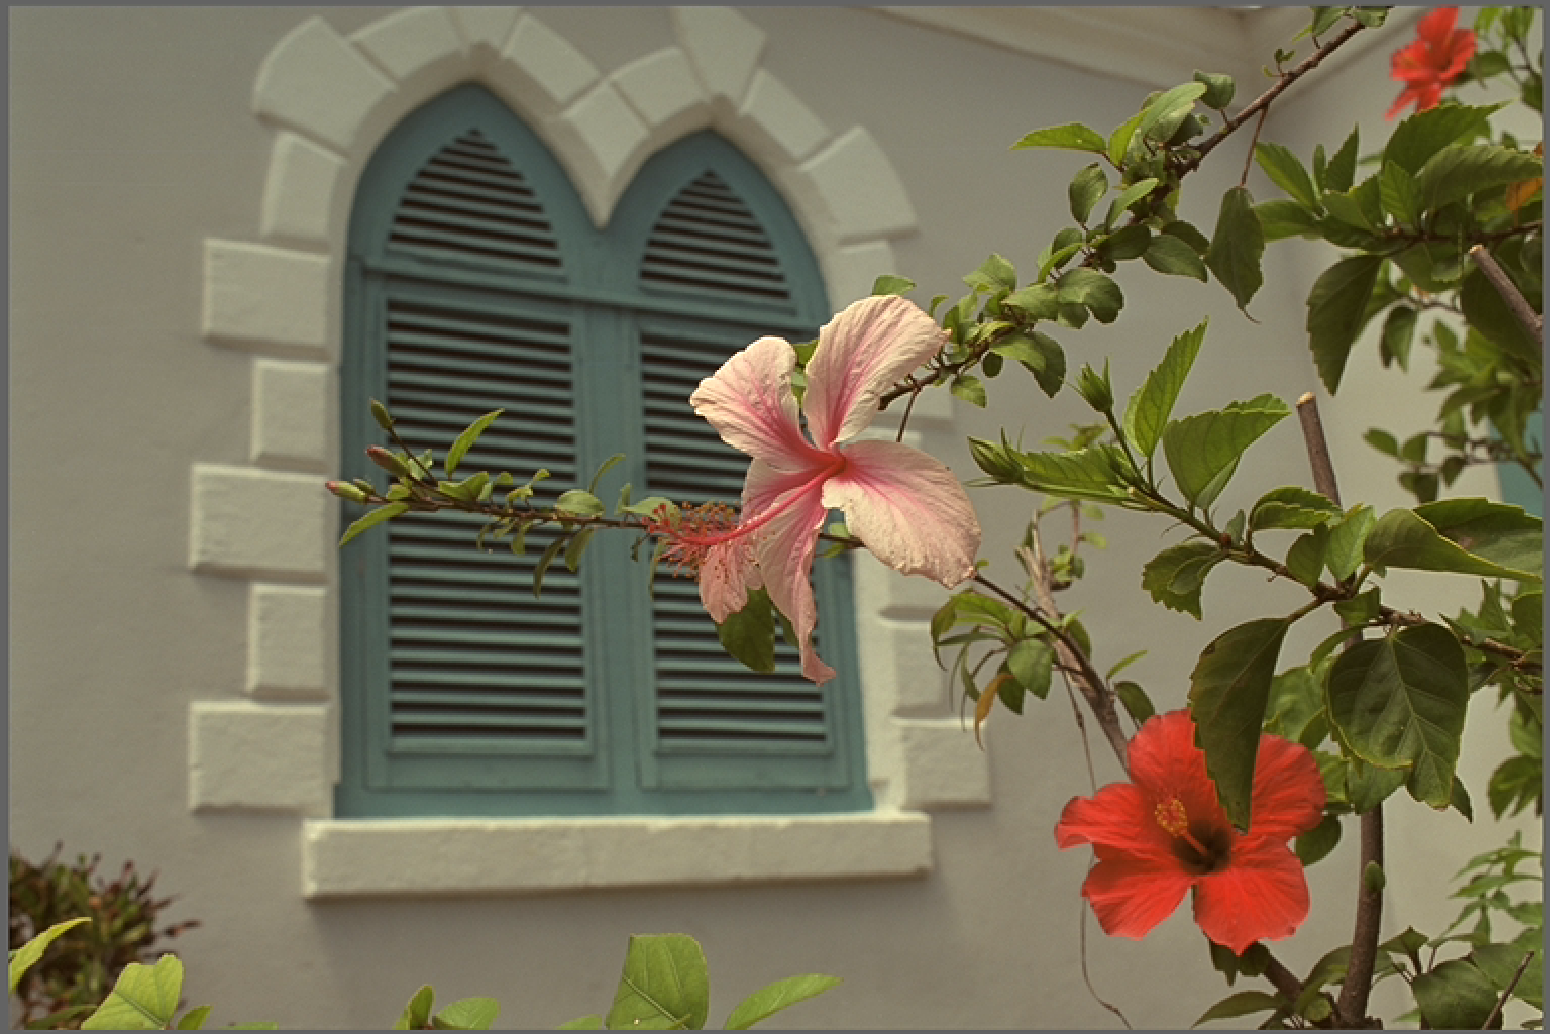
\includegraphics[scale=0.33]{../img/toyaref07.pdf}
    \legend{Fonte: \cite{Tourancheau2008}}
  \end{minipage}
  \hfill
  \begin{minipage}{0.45\textwidth}
    \centering
    \caption{Imagem distorcida Toyama} \label{fig:toyadist}
    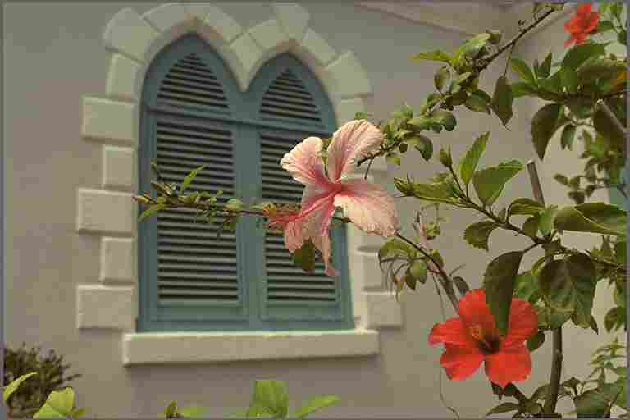
\includegraphics[scale=0.80]{../img/toyadist07_79.pdf}
    \legend{Fonte: \cite{Tourancheau2008}}
  \end{minipage}
\end{figure}
